\section{Preliminaries}
\label{sec:preliminaries}

This section introduces the fundamental concepts and definitions required to
understand the remainder of this thesis. It establishes the formal game-theoretic
model of chess, derives the associated search problem, and motivates the use of
heuristic evaluation and time-constrained search. All concepts presented in this
section are standard in the field of computer chess and provide a common basis
for the subsequent chapters.

\subsection{Chess as a Game-Theoretic Model}

Chess is modeled as a deterministic, two-player, zero-sum game with perfect
information. At any point in time, the complete game state is fully observable
to both players, and no randomness is involved in the game mechanics.

A game state consists of a board configuration together with additional state
information such as the side to move, castling rights, and en-passant
availability. Players alternate turns by selecting legal moves, and the game
terminates in a win, loss, or draw according to the rules of chess.

More formally, let $\mathcal{T} = \{\text{pawn}, \text{knight}, \text{bishop},
\text{rook}, \text{queen}, \text{king}\}$ denote the set of piece types and
$\mathcal{C} = \{\text{white}, \text{black}\}$ the set of colours. A piece is then
an element of $\mathcal{F} = \mathcal{T} \times \mathcal{C}$, and the placement of
pieces on the board is described by a mapping
\[
b : \{1, \dots, 8\}^2 \rightarrow \mathcal{F} \cup \{\varnothing\},
\]
which assigns to each square either a piece or the empty symbol $\varnothing$. A
complete game state $s = (b, t, r, e)$ additionally comprises the side to move
$t \in \mathcal{C}$, the castling rights $r$, and the en-passant target $e$, both
of which depend on the movement history rather than on the current placement
alone. The set of all legal states is denoted by $\mathcal{S}$.

The rules of chess induce a transition relation
$\delta \subseteq \mathcal{S} \times \mathcal{S}$, where $(s, s') \in \delta$ if
and only if $s'$ can be reached from $s$ by exactly one legal move. This relation
defines a directed graph $G = (\mathcal{S}, \delta)$ in which each node is a legal
position and each edge is a legal move. A state $s$ is \emph{terminal} if it has
no outgoing edges, as in checkmate or stalemate, or if it is declared drawn by
the rules of chess.

For decision making, the graph $G$ is unrolled into a game tree rooted at the
current position. Each level of the tree corresponds to one ply, and the number of
nodes per level is governed by the branching factor of chess, which amounts to
around $30$ available actions per position~\cite{yannakakis2018artificial}.

\subsection{Search Problem Formulation}

Given a current position, the task of a chess engine is to select a legal move
that maximizes the expected outcome under the assumption of optimal play by both
sides. In the classical formulation, the possible outcomes are associated with
numerical values, for example $+1$ for a win, $0$ for a draw, and $-1$ for a
loss.

This decision problem is commonly formulated as a game tree search problem, in
which the engine explores a subset of the game tree to estimate the value of
available moves. The root of the tree corresponds to the current position, while
internal nodes represent positions reachable through sequences of legal moves.

With that branching factor the tree grows exponentially with depth, so evaluating
all reachable positions is computationally infeasible even for moderate depths.
Consequently, the search must be limited by depth,
time, or other computational resources. This limitation introduces approximation:
the engine can no longer guarantee optimal play, but instead aims to select the
best move according to the information explored within the available budget.

The quality of a move selected by a chess engine therefore depends on two main
factors: the effectiveness of the search algorithm in selecting which parts of
the tree to explore, and the accuracy of the evaluation function used to estimate
the value of positions at the search frontier.

\subsection{Minimax, Negamax, Quiescence and Alpha-Beta Pruning}
\label{subsec:minimax_alphabeta}

The classic algorithmic solution to game tree search in two-player zero-sum
games with perfect information is the Minimax algorithm. Minimax assumes that
one player aims to maximize the evaluation value of a position, while the
opponent aims to minimize it. Terminal positions are assigned fixed values
corresponding to win, loss, or draw, while non-terminal leaf positions are
evaluated heuristically.

The algorithm explores the game tree recursively and propagates values from the
leaves toward the root by alternating between maximization and minimization
steps. A detailed introduction to Minimax can be found in standard textbooks on
artificial intelligence in games, such as Yannakakis and
Togelius~\cite{yannakakis2018artificial}.

\paragraph{Negamax Formulation}
In zero-sum games, the Minimax algorithm can be simplified using the Negamax
formulation. Instead of explicitly distinguishing between maximizing and
minimizing players, Negamax expresses all evaluations from the perspective of the
side to move. The value of a position is defined as the negation of the value
obtained by the opponent after making a move.

This formulation exploits the symmetry of \emph{two-player} zero-sum games, in
which one side's gain is exactly the other's loss, so that a single score suffices
if it is always read from the perspective of the side to move. It allows the
search to be implemented using a single recursive procedure. Negamax is
functionally equivalent to Minimax but leads to more compact and uniform code,
which is why it is widely used in practical chess engines.

\paragraph{Quiescence Search}
Depth-limited game tree search combined with static evaluation functions suffers
from a well-known problem referred to as the \emph{horizon effect}. Tactical
events such as captures, checks, or promotions may occur just beyond the search
depth and are therefore not accounted for by the evaluation function. As a
result, the engine may incorrectly assess positions as stable even though
significant tactical changes are imminent.

Quiescence search is a standard technique to solve this problem. Instead of
evaluating a position immediately when the nominal search depth is reached, the
search is selectively extended in positions that are considered tactically
unstable. Typically, only forcing moves such as captures or checking moves are
explored, while quiet moves are excluded.

The goal of quiescence search is to reach a \emph{quiescent} position, that is, a
position in which no immediate tactical exchanges are available and the static
evaluation is therefore more reliable. Once such a position is reached, the
evaluation function is applied and the resulting score is propagated back up the
search tree.

\cref{fig:horizon} shows why a fixed depth limit is not merely imprecise but can
be actively misleading. An exchange of pieces unfolds over several plies, and its
intermediate states are wildly unbalanced: after one side has captured but before
the recapture, the position looks winning by a whole piece. A search that stops
exactly at that moment reports this intermediate state as the final one. The
error is not small and random but large and systematic, since it always favors
the side that captured last. This is also the reason a purely depth-based
comparison of search algorithms is fragile without quiescence search, as one
additional ply can invert the sign of the evaluation.

\begin{figure}[ht]
\centering
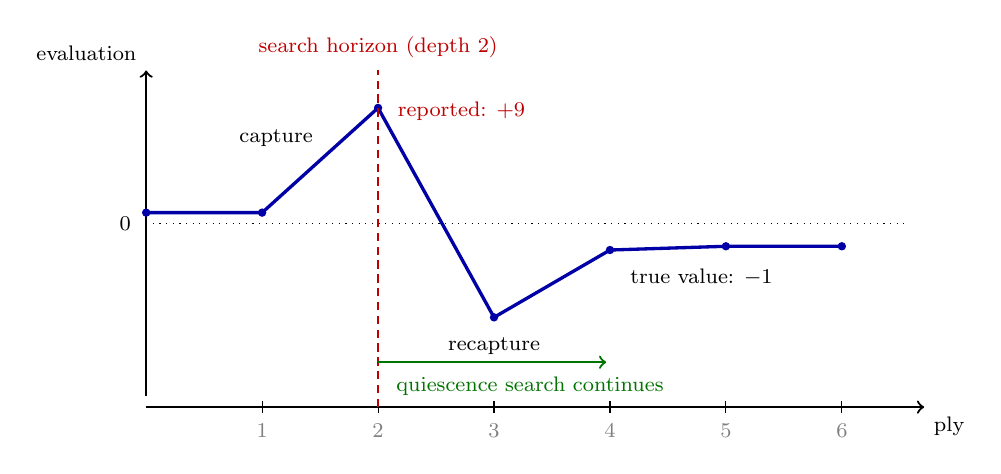
\begin{tikzpicture}[scale=0.95, transform shape, font=\small]
% evaluation axis (zero line kept separate from the ply axis)
\draw[->, thick] (0,-2.3) -- (0,2.05) node[above left, font=\footnotesize] {evaluation};
\draw[dotted] (0,0) -- (10.2,0);
\node[font=\footnotesize, anchor=east] at (-0.08,0) {$0$};

% ply axis, drawn below the curve so labels never touch it
\draw[->, thick] (0,-2.45) -- (10.4,-2.45) node[below right, font=\footnotesize] {ply};
\foreach \x/\lab in {1/1,2/2,3/3,4/4,5/5,6/6}{
  \draw (1.55*\x,-2.37) -- (1.55*\x,-2.53);
  \node[below, font=\footnotesize, gray] at (1.55*\x,-2.55) {\lab};
}

% evaluation trace: quiet, capture (+9), recapture (-1), quiet
\coordinate (p0) at (0,0.15);
\coordinate (p1) at (1.55,0.15);
\coordinate (p2) at (3.10,1.55);
\coordinate (p3) at (4.65,-1.25);
\coordinate (p4) at (6.20,-0.35);
\coordinate (p5) at (7.75,-0.30);
\coordinate (p6) at (9.30,-0.30);
\draw[very thick, blue!65!black] (p0) -- (p1) -- (p2) -- (p3) -- (p4) -- (p5) -- (p6);
\foreach \p in {p0,p1,p2,p3,p4,p5,p6}
  \fill[blue!65!black] (\p) circle (1.6pt);

% horizon at ply 2
\draw[red!75!black, thick, densely dashed] (3.10,-2.45) -- (3.10,2.05);
\node[red!75!black, font=\footnotesize, anchor=south] at (3.10,2.10)
  {search horizon (depth 2)};
\node[red!75!black, font=\footnotesize, anchor=west] at (3.24,1.50)
  {reported: $+9$};

% quiescence extension
\draw[->, green!45!black, thick] (3.10,-1.85) -- (6.15,-1.85);
\node[green!45!black, font=\footnotesize, anchor=north west] at (3.22,-1.92)
  {quiescence search continues};
\node[font=\footnotesize, anchor=west] at (6.35,-0.72) {true value: $-1$};

% annotations on the trace
\node[font=\footnotesize, anchor=east] at (2.35,1.15) {capture};
\node[font=\footnotesize, anchor=north] at (4.65,-1.40) {recapture};
\end{tikzpicture}
\caption{The horizon effect. The curve shows the static evaluation along a single
line of play in which a capture is answered by a recapture. A search limited to
two plies stops immediately after the capture and reports a decisive material
advantage that does not exist; one ply later the material is nearly balanced
again. Quiescence search resolves this by continuing beyond the nominal depth as
long as captures are available, and evaluating only once the position is quiet.}
\label{fig:horizon}
\end{figure}

In practice, quiescence search is commonly implemented using Alpha-Beta pruning
with a so-called \emph{stand-pat} evaluation~\cite{marsland1986review}, which
represents the static evaluation of the current position before any tactical
extensions are explored. If the stand-pat score already exceeds the current
bounds, the node can be pruned early.

Quiescence search significantly improves evaluation stability in tactical
positions and has become a standard component of classical chess engines. A
comprehensive discussion of the horizon effect and quiescence search can be
found in survey articles on game tree pruning~\cite{marsland1986review}.

\paragraph{Alpha-Beta Pruning}
Alpha-Beta pruning is an optimization technique that reduces the number of nodes
that need to be explored by Minimax or Negamax without affecting the correctness
of the final result. The technique was introduced by Knuth and Moore~\cite{knuth1975alphabeta}
and is a cornerstone of modern game tree search.

The algorithm maintains two bounds during search:
\begin{itemize}
    \item $\alpha$, the best score that the maximizing player can guarantee so
    far,
    \item $\beta$, the best score that the minimizing player can guarantee so
    far.
\end{itemize}

At the root of the search tree, $\alpha$ is initialized to $-\infty$ and $\beta$
to $+\infty$. As the search progresses, these bounds are updated based on the
values of explored child nodes. Whenever a node is encountered for which it can
be shown that its value cannot improve the current result, the corresponding
subtree is pruned and not searched further.

More concretely, during a maximizing step, the value of $\alpha$ is updated
whenever a better move is found. If $\alpha$ becomes greater than or equal to
$\beta$, further exploration of sibling nodes is unnecessary, as the minimizing
player would avoid reaching this position. An analogous argument applies during
minimizing steps.

\cref{fig:alphabeta} illustrates this on a minimal tree. The essential point is
that the pruned subtree is discarded without being looked at, and that this is
nevertheless safe: the discarded branch contains the highest leaf value of the
entire tree, but that value is never reachable, because the opponent decides at
that node and already holds a better alternative there. Pruning therefore removes
work, not information, which is what distinguishes Alpha-Beta from the heuristic
pruning discussed in \cref{subsec:null_move_pruning}.

\begin{figure}[ht]
\centering
\begin{tikzpicture}[
  scale=0.95, transform shape,
  font=\small,
  maxn/.style={draw, thick, rectangle, minimum size=8mm, inner sep=1pt},
  minn/.style={draw, thick, circle, minimum size=8mm, inner sep=1pt},
  leaf/.style={draw, rectangle, rounded corners=2pt, minimum size=7mm, inner sep=2pt},
  gone/.style={draw=gray!50, densely dashed, rectangle, rounded corners=2pt,
               minimum size=7mm, inner sep=2pt, text=gray!60},
  edge/.style={-, thick},
  gedge/.style={-, gray!50, densely dashed}
]
% --- nodes -----------------------------------------------------------------
\node[maxn] (root) at (5,3.1) {$5$};
\node[left=1mm of root, font=\footnotesize] {MAX};

\node[minn] (a) at (1.7,1.5) {$5$};
\node[minn] (b) at (5,1.5)   {$\leq 3$};
\node[minn] (c) at (8.3,1.5) {$4$};
\node[left=1mm of a, font=\footnotesize] {MIN};

\node[leaf] (a1) at (0.8,0) {$5$};
\node[leaf] (a2) at (2.6,0) {$6$};
\node[leaf] (b1) at (4.1,0) {$3$};
\node[gone] (b2) at (5.0,0) {$8$};
\node[gone] (b3) at (5.9,0) {$2$};
\node[leaf] (c1) at (7.4,0) {$7$};
\node[leaf] (c2) at (9.2,0) {$4$};

% --- edges -----------------------------------------------------------------
\foreach \t in {a,b,c} \draw[edge] (root) -- (\t);
\foreach \t in {a1,a2} \draw[edge] (a) -- (\t);
\draw[edge] (b) -- (b1);
\foreach \t in {b2,b3} \draw[gedge] (b) -- (\t);
\foreach \t in {c1,c2} \draw[edge] (c) -- (\t);

% --- cut marker ------------------------------------------------------------
\draw[red!75!black, thick] (4.85,0.78) -- (5.68,0.78);
\node[red!75!black, font=\footnotesize, anchor=west] at (5.78,0.78) {cutoff};
\node[font=\footnotesize, align=center, anchor=north] at (5.0,-0.55)
  {not searched\\[-1pt]$\beta = 3 \leq \alpha = 5$};
\node[font=\footnotesize, align=left, anchor=east] at (1.05,2.35)
  {$\alpha = 5$};
\end{tikzpicture}
\caption{Alpha-Beta pruning on a minimal tree. The square root node maximizes,
the circular nodes minimize. The left subtree is searched first and yields $5$,
so the maximizing player is guaranteed at least $\alpha = 5$. In the middle
subtree the first leaf already returns $3$; since the minimizing player will
never choose more than $3$ there, this subtree cannot beat $5$ and its remaining
leaves are skipped, including the $8$, which is the largest value in the whole
tree. The result is identical to an exhaustive search, but two of the seven
leaves are never evaluated.}
\label{fig:alphabeta}
\end{figure}

\paragraph{Effectiveness and Influencing Factors}
In the worst case, Alpha-Beta pruning explores the same number of nodes as plain
Minimax. However, with optimal move ordering, the effective branching factor is
significantly reduced, allowing the search to reach roughly twice the depth of
unpruned Minimax for the same computational effort.

The effectiveness of Alpha-Beta pruning therefore depends strongly on the order
in which moves are explored. Techniques such as heuristic move ordering,
transposition tables, and iterative deepening are commonly employed to improve
this order and thereby increase pruning efficiency. These aspects are discussed
in more detail in \cref{sec:algorithm_implementation}.

\paragraph{Principal Variation Search}
Principal Variation Search (PVS) is a refinement of Alpha-Beta pruning that
exploits good move ordering even further~\cite{marsland1982parallel,
pearl1980scout}. The technique is based on the assumption that the first move
examined at a node is usually the best one. Only this first move is searched
with the full window $[\alpha, \beta]$. Every remaining move is first examined
with a so-called \emph{null window} (or zero window) $[\alpha, \alpha + 1]$,
which cannot return an exact score but can cheaply prove whether the move has
the potential to improve upon $\alpha$.

If the null-window search fails low, the move is confirmed to be inferior to
the current best move and no further work is required. If it fails high, the
assumption was wrong: the move may be better than the principal variation, and
the node must be \emph{re-searched} with the full window to obtain its exact
score. PVS therefore trades occasional re-searches for substantially cheaper
verification of the majority of moves. With strong move ordering, fail-highs
are rare and the technique reduces the overall search effort
considerably~\cite{reinefeld1983negascout}. Conversely, with poor move
ordering, frequent re-searches can negate the savings, which is why PVS is
typically combined with iterative deepening, transposition tables, and
heuristic move ordering.

For a comprehensive discussion of Alpha-Beta pruning and its variants in the
context of game-playing programs, see Marsland~\cite{marsland1986review}.

\subsection{Heuristic Evaluation}

Most positions encountered during search are non-terminal and therefore cannot be
assigned an exact game-theoretic value. Instead, they must be evaluated
heuristically. An evaluation function assigns a numerical score to a position,
indicating its desirability from the perspective of the side to move.

Classical evaluation functions combine material considerations with positional
features such as piece activity, king safety, and pawn structure. These features
are typically handcrafted and encode domain knowledge about the game of chess.
The design of the evaluation function has a significant impact on the playing
strength of the engine, particularly when search depth is limited.

Conceptually, the score returned by an evaluation function is expressed in a
common unit, most often \emph{centipawns}, where one pawn corresponds to a value
of $100$. Expressing heterogeneous factors, such as material imbalance and
positional advantages, on a single comparable scale allows them to be combined
into one number that the search can compare consistently across positions.

A refinement that is widely used in classical engines is the \emph{tapered}
evaluation. Since the relative importance of individual features changes over the
course of a game, for example when kings become active in the endgame, the
evaluation maintains two scores, one tuned for the midgame and one for the
endgame, and interpolates between them according to a game-phase measure derived
from the remaining material. The concrete evaluation used in this thesis follows
exactly this scheme and is described in detail in \cref{sec:evaluation_function}.

Finally, there is an inherent tension between the richness of the evaluation and
the depth of the search. A more detailed evaluation captures more chess knowledge
per node but is more expensive to compute, which reduces the number of nodes that
can be searched within a fixed time budget.

\subsection{Time-Constrained Search}

In practical settings, chess engines are required to operate under strict time
constraints. Rather than searching to a fixed depth, the engine must dynamically
adapt its search behavior to the available time budget.

\paragraph{Iterative Deepening}
Iterative deepening addresses this requirement by turning a single fixed-depth
search into a sequence of searches with increasing depth limit
$d = 1, 2, 3, \dots$, each starting again from the root~\cite{korf1985iterative}.
After every completed iteration the engine holds a fully valid best move for that
depth, so the search can be interrupted at essentially any point and still return
a well-founded decision. This \emph{anytime} property is precisely what makes the
technique well suited to time-controlled play, where the exact amount of
available time is not known in advance.

At first glance, repeatedly re-searching the shallow part of the tree appears
wasteful. In practice the overhead is small: because the number of nodes grows
exponentially with depth, the cost of the final iteration dominates the sum of
all previous ones, so re-searching depths $1$ to $d-1$ adds only a constant
factor to the cost of the depth-$d$ search. As discussed next, this overhead is
typically more than recovered through the improved move ordering that earlier
iterations provide.

\cref{fig:iterative_deepening} makes the two consequences of this exponential
growth visible at once. Because each iteration costs roughly three times its
predecessor, everything before the last one is nearly free, which is what makes
the repetition affordable. The same fact, however, means the engine faces an
all-or-nothing decision at every iteration boundary: the next iteration will
consume more time than the entire search so far, and if the clock runs out
half-way through it, that work is discarded entirely. Deciding whether to start
another iteration is therefore not a minor scheduling detail but the central
question of time management, and it is addressed in
\cref{sec:time_management}.

\begin{figure}[ht]
\centering
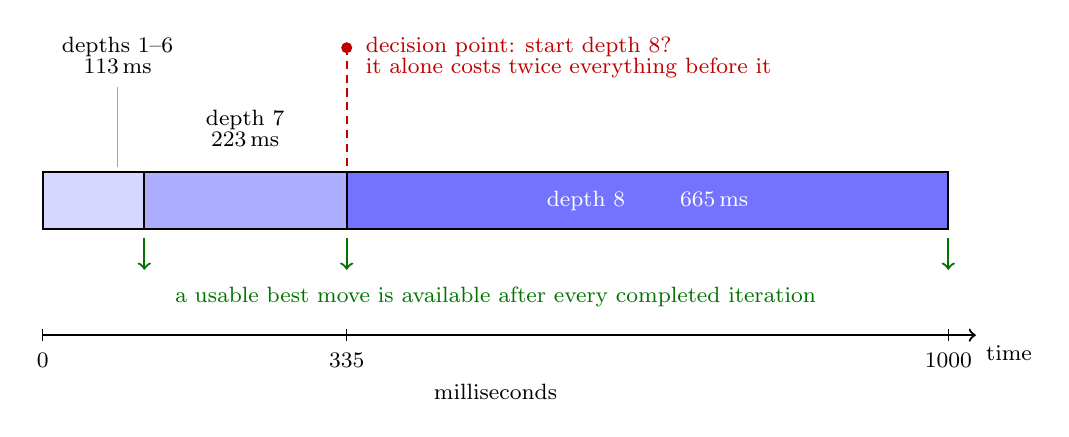
\begin{tikzpicture}[scale=1.0, font=\small]
% ---- the bar: widths proportional to measured cost per iteration ----------
\def\ybot{0}\def\ytop{0.72}
\fill[blue!16] (0,\ybot)    rectangle (1.29,\ytop);
\fill[blue!32] (1.29,\ybot) rectangle (3.86,\ytop);
\fill[blue!55] (3.86,\ybot) rectangle (11.5,\ytop);
\draw[thick] (0,\ybot) rectangle (11.5,\ytop);
\foreach \x in {1.29,3.86} \draw[thick] (\x,\ybot) -- (\x,\ytop);

% ---- segment labels ------------------------------------------------------
\node[font=\footnotesize, white] at (7.68,0.36) {depth 8 \qquad $665$\,ms};
\node[font=\footnotesize, align=center, anchor=south] at (2.57,0.92)
  {depth 7\\[-2pt]$223$\,ms};
\node[font=\footnotesize, align=center, anchor=south] at (0.95,1.85)
  {depths 1--6\\[-2pt]$113$\,ms};
\draw[gray!70] (0.95,1.80) -- (0.95,0.78);

% ---- time axis -----------------------------------------------------------
\draw[->, thick] (0,-1.35) -- (11.85,-1.35) node[below right, font=\footnotesize] {time};
\foreach \x/\lab in {0/0, 3.86/335, 11.5/1000}{
  \draw (\x,-1.27) -- (\x,-1.43);
  \node[below, font=\footnotesize] at (\x,-1.45) {\lab};
}
\node[below, font=\footnotesize] at (5.75,-1.85) {milliseconds};

% ---- soft stop decision --------------------------------------------------
\draw[red!75!black, thick, densely dashed] (3.86,\ytop+0.08) -- (3.86,2.30);
\fill[red!75!black] (3.86,2.30) circle (2pt);
\node[red!75!black, font=\footnotesize, anchor=south west, align=left]
  at (3.98,1.80) {decision point: start depth 8?\\[-2pt]
                  it alone costs twice everything before it};

% ---- anytime property ----------------------------------------------------
\foreach \x in {1.29,3.86,11.5}
  \draw[->, green!45!black, thick] (\x,-0.12) -- (\x,-0.52);
\node[green!45!black, font=\footnotesize, anchor=north] at (5.75,-0.62)
  {a usable best move is available after every completed iteration};
\end{tikzpicture}
\caption{Iterative deepening under a one-second budget, with the width of each
segment proportional to the time that iteration consumes. The proportions follow
from the effective branching factor of about $3$ measured for this engine in
\cref{subsec:eval_ttq}. The first six iterations together account for roughly a
tenth of the budget, so the repeated re-searching is cheap; the last iteration
alone accounts for two thirds. Every completed iteration leaves a valid best move
behind, which is what allows the search to be stopped at any point.}
\label{fig:iterative_deepening}
\end{figure}

\paragraph{Interaction with Pruning}
In addition to providing robustness under time constraints, iterative deepening
also improves the effectiveness of Alpha-Beta pruning. Information gathered in
earlier iterations, such as good move orderings, can be reused in deeper searches,
leading to a significant reduction in the number of explored nodes.

\paragraph{Search Tree Reuse Across Searches}
The same principle extends beyond a single search invocation. After the engine
has played a move and the opponent has responded, the new search root lies
within the tree that was explored during the previous search. If the results of
that search are retained, for example in a transposition table, the engine can
\emph{resume} the old search tree: previously computed scores yield immediate
cutoffs, and previously identified best moves improve the move ordering from the
very first iteration. Conceptually, the engine no longer starts each search from
scratch but continues the computation it has already begun in earlier moves of
the game.

The interaction between heuristic evaluation, Alpha-Beta pruning, and
time-constrained iterative deepening forms the foundation of modern chess
engines and is a central aspect of this work.